\documentclass[11pt]{article}
\usepackage[utf8]{inputenc}
\usepackage[T1]{fontenc}
\usepackage{graphicx}
\usepackage{grffile}
\usepackage{longtable}
\usepackage{wrapfig}
\usepackage{rotating}
\usepackage[normalem]{ulem}
\usepackage{amsmath}
\usepackage{textcomp}
\usepackage{amssymb}
\usepackage{capt-of}
\usepackage{hyperref}
\usepackage{minted}
\author{Student: Brian Cheung bc32427 \\ Professor: Mohit Tiwari \\ TA: Antonio Espinoza \\ Department of Electrical \& Computer Engineering \\ The University of Texas at Austin}
\date{\today}
\title{EE379K Enterprise Network Security Lab 1 Report}
\hypersetup{
 pdfauthor={Student: Brian Cheung bc32427 \\ Professor: Mohit Tiwari \\ TA: Antonio Espinoza \\ Department of Electrical \& Computer Engineering \\ The University of Texas at Austin},
 pdftitle={EE379K Enterprise Network Security Lab 1 Report},
 pdfkeywords={},
 pdfsubject={},
 pdfcreator={},
 pdflang={English}}
\begin{document}

\maketitle
\section{Part 1}
\label{sec:part-1}
part 1 paragraph
\subsection{Step 1 - Echo Server}
\subsubsection{Build server and client}
In a terminal window, start at root directory of project and run the following commands:
\begin{minted}{bash}
  $ cd Part\ 1
  $ make
\end{minted}
\subsubsection{Run server and client}
Run the following commands to start the server:
\begin{minted}{bash}
  $ cd Part\ 1
  $ ./server
\end{minted}
Open a new terminal window and run the following commands to start the client:
\begin{minted}{bash}
  $ cd Part\ 1
  $ ./client
\end{minted}
\subsection{Step 2 - DOS Attack}
The DOS attack was performed using a program called \textbf{\emph{hping3}}.
The attacker flooded the server with SYN packets while using a spoofed IP address to hide the source IP address.
Without the correct IP, the server was unable to send SYN and ACK packets back to the attacker,
which prevented the three-way handshake from being completed.
By flooding the server with SYN packets and preventing the three-way handshake from being completed,
the server cannot process other clients' requests because it is too busy trying to complete the attacker's requests,
so clients that want to connect to the server are left waiting.

\noindent The following command was used to perform the DOS attack:
\begin{minted}{bash}
  $ sudo hping3 -S -w 64 -p 12000 --flood --rand-source 127.0.0.2
\end{minted}
\textbf{\emph{hping3}} command flags and options:

\textbf{-S}: flood with SYN packets

\textbf{-p}: 12000: port 12000

\textbf{--flood}: send packets as fast as possible

\textbf{--rand-source}: generates a spoofed IP address to hide the source IP

\textbf{127.0.0.2}: IP address of server

\section{Part 2}
\label{sec:part-2}
part 2 paragraph

Example Figure \ref{fig:rocc-encoding} shows X. Example reference to paper~\cite{Brasser17}.

\begin{figure}[htbp]
\centering
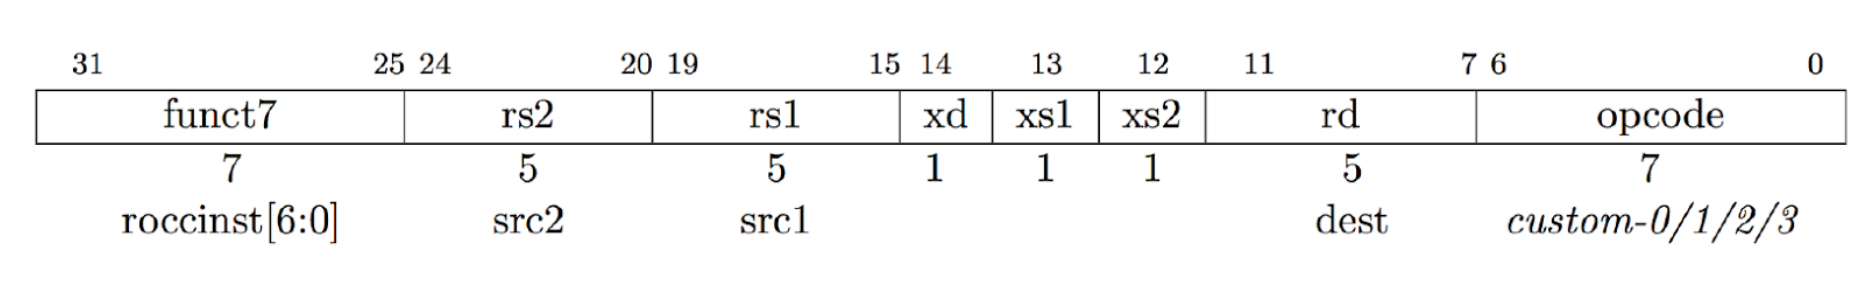
\includegraphics[width=.9\linewidth]{./rocc-encoding.png}
\caption{\label{fig:rocc-encoding}
The RoCC Accelerator Instruction Encoding}
\end{figure}
\section{Part 3}

\label{sec:part-3}
part 3 paragraph

\begin{minted}{c++}
  int main() {
    printf("Hello World");
    return 0;
  }
\end{minted}

\section{Part 4}
\label{sec:part-4}

\section{Conclusion}
\label{sec:conclusion}
Please provide feedback so we can improve the labs for the course. How many
hours did the lab take you? Was this lab boring? Did you learn anything? Is
there anything you would change? Feel free to put anything here, but leaving it
blank will result in the loss of points.

\bibliography{bibliography}
\bibliographystyle{ieeetr}
\end{document}
